\documentclass[a0paper,portrait]{baposter}

\usepackage[utf8]{inputenc}
\usepackage[spanish]{babel}
\usepackage{graphicx}
\usepackage{grffile} 
\graphicspath{{figures/}} 
\usepackage{amsmath}
\usepackage{amssymb}
\usepackage{xcolor}
\usepackage{tikz}
\usepackage{circuitikz}
\usepackage{multicol}
\usepackage{enumitem}

% --- DEFINICIÓN DE COLORES ---
\definecolor{emptyColor}{HTML}{475569}
\definecolor{bots25Color}{HTML}{0284C7}
\definecolor{bots26Color}{HTML}{D97706}
\definecolor{bots27Color}{HTML}{BE123C}
\definecolor{sageGreenDark}{HTML}{4A5D4A}
\definecolor{sageGreenLight}{HTML}{B5C7B5}
\definecolor{boxColor}{HTML}{FFFFFF}
\definecolor{headerColor}{HTML}{3A4A3A}

\begin{document}
	
	% --- CONFIGURACIÓN MINIMALISTA Y A PRUEBA DE FALLOS ---
	\begin{poster}{
			grid=false,
			columns=6,
			colspacing=1em,
			background=none,
			bgColorOne=white,
			borderColor=sageGreenDark,
			headerColorOne=headerColor,
			headerFontColor=white,
			boxColorOne=white
		}
		% --- LOGO IZQUIERDO ---
		{
\includegraphics[width=8cm]{logoITBA.png}}
		% --- TÍTULO ---
		{\vspace{0.3em} \huge \textbf{Medición de presión en sistemas de partículas autopropulsadas\\[0.1em] confinadas mediante sensores FSR en configuración integral y distribuida}\vspace{0.3em}}
		% --- AUTORES ---
		{\large \textbf{Dylan Frigerio $^{1}$, German Patterson $^{1,2}$} \\[0.1em] 
			\normalsize $^{1}$ Instituto Tecnológico de Buenos Aires (ITBA), $^{2}$ CONICET | dyfrigerio@itba.edu.ar}
		% --- LOGO DERECHO ---
		{
\includegraphics[width=8cm]{logoCONICET.png}}
		
		
		% ==========================================
		% INTRODUCCIÓN (Ancha y corta)
		% ==========================================
		\begin{posterbox}[name=intro,column=0,span=6,row=0]{1. RESUMEN DEL PROYECTO}
			\large \textbf{Objetivo:} Desarrollar un sensor FSR de bajo costo para medir la presión integral y distribuida ejercida por Kilobots en un recinto circular. Buscamos relacionar directamente la densidad del enjambre ($N$) con las fluctuaciones espaciales de fuerza y los ciclos temporales de atasco (\textit{jamming}) que se producen por el confinamiento geométrico de la materia activa.
		\end{posterbox}
		
		
		% ==========================================
		% COLUMNA IZQUIERDA (Setup, Futuro, Leyenda, Refs)
		% ==========================================
		\begin{posterbox}[name=setup,column=0,span=2,below=intro]{2. SETUP EXPERIMENTAL (INTEGRAL)}
			\textbf{Parámetros:} $N \in \{0, 25, 26, 27\}$ bots | 20 Hz | 30 min.
			
			\vspace{0.4em}
			\centering
			\includegraphics[width=0.48\textwidth]{Kilobot.jpeg} \hfill
			\includegraphics[width=0.48\textwidth]{fsr408.jpg}\\
			\vspace{0.2em}
			{\small \textit{Izq: Kilobots. Der: Cinta Sensora FSR perimetral.}}
			
			\vspace{0.6em}
			\resizebox{0.9\textwidth}{!}{
				\shorthandoff{>}
				\begin{circuitikz}[american, scale=0.8, transform shape]
					\draw (0,0) node[op amp] (opamp) {};
					\draw (opamp.-) to[R, l=$R_{in}$] (-3, 0.5) node[left] {$V_{exc}$};
					\draw (opamp.+) -- ++(0,-0.5) node[ground] {};
					\draw (opamp.-) -- ++(0,1.5) coordinate (fb) to[vR, l=FSR] (fb -| opamp.out) -- (opamp.out);
					\draw (opamp.out) to[short, -o] ++(1,0) node[right, text width=2.5cm, align=left] {MCU 10-bit ADC\\UART 115200bps};
				\end{circuitikz}
				\shorthandon{>}
			}\\
			\vspace{0.2em}
			{\small \textit{Circuito inversor ($V_{exc}=-0.75V$) actual.}}
		\end{posterbox}
		
		% --- TRABAJO FUTURO: CONFIGURACIÓN ESPACIAL (MUX + OpAmps) ---
		\begin{posterbox}[name=futuro,column=0,span=2,below=setup]{3. TRABAJO FUTURO: MEDICIÓN ESPACIAL}
			\small \textbf{Configuración Distribuida:} Para mapear la inhomogeneidad de fuerzas, la cinta se seccionará en múltiples recortes independientes.
			
			\vspace{0.6em}
			\centering
			\resizebox{0.95\textwidth}{!}{%
				\shorthandoff{>}%
				\begin{tikzpicture}[>=stealth, node distance=1.6cm, auto]
					% Sensores
					\node[draw, fill=sageGreenLight, minimum width=1.5cm] (fsr1) {FSR 1};
					\node[below of=fsr1, yshift=0.8cm] (dots) {$\vdots$};
					\node[draw, fill=sageGreenLight, minimum width=1.5cm, below of=dots, yshift=0.8cm] (fsrn) {FSR N};
					
					% OpAmps
					\node[draw, right of=fsr1, xshift=0.6cm] (op1) {OpAmp};
					\node[draw, right of=fsrn, xshift=0.6cm] (opn) {OpAmp};
					
					% MUX y ADC
					\node[draw, fill=emptyColor!20, minimum height=2.8cm, right of=op1, xshift=1.2cm, yshift=-0.8cm] (mux) {MUX};
					\node[draw, right of=mux, xshift=0.5cm] (adc) {ADC};
					
					% Conexiones
					\draw[->, thick] (fsr1) -- (op1);
					\draw[->, thick] (fsrn) -- (opn);
					\draw[->, thick] (op1) -- (op1 -| mux.west);
					\draw[->, thick] (opn) -- (opn -| mux.west);
					\draw[->, thick, double] (mux) -- (adc);
				\end{tikzpicture}%
				\shorthandon{>}%
			}
			\vspace{0.2em}\\
			{\small \textit{Acondicionamiento dedicado por canal, multiplexado para lectura secuencial vía ADC.}}
		\end{posterbox}
		
		\begin{posterbox}[name=legend,column=0,span=2,below=futuro]{LEYENDA: DENSIDAD ($N$)}
			\centering
			\begin{tikzpicture}
				\matrix [column sep=5mm, row sep=2mm] {
					\fill[emptyColor] (0,0) rectangle (0.5,0.5); \node[right] at (0.5,0.25) {Empty (0)}; &
					\fill[bots25Color] (0,0) rectangle (0.5,0.5); \node[right] at (0.5,0.25) {25 bots}; \\
					\fill[bots26Color] (0,0) rectangle (0.5,0.5); \node[right] at (0.5,0.25) {26 bots}; &
					\fill[bots27Color] (0,0) rectangle (0.5,0.5); \node[right] at (0.5,0.25) {27 bots}; \\
				};
			\end{tikzpicture}
		\end{posterbox}
		
		\begin{posterbox}[name=refs,column=0,span=2,below=legend]{REFERENCIAS}
			\raggedright
			\scriptsize
			[1] AP Solon et al., Nature Physics 11 (2015) 673.\\[0.2em]
			[2] G Junot et al., Phys. Rev. Lett. 119 (2017) 028002.\\[0.2em]
			[3] GA Patterson et al., Phys. Rev. Lett. 119 (2017) 248301.\\[0.2em]
			[4] MR Ferressini et al., Phys. Rev. E (2025) 015406.
		\end{posterbox}
		
		
		% ==========================================
		% COLUMNAS DERECHAS (Resultados)
		% ==========================================
		\begin{posterbox}[name=hist,column=2,span=4,below=intro]{A. Distribución de Presión: Máxima Asimetría ($N=27$)}
			\centering
			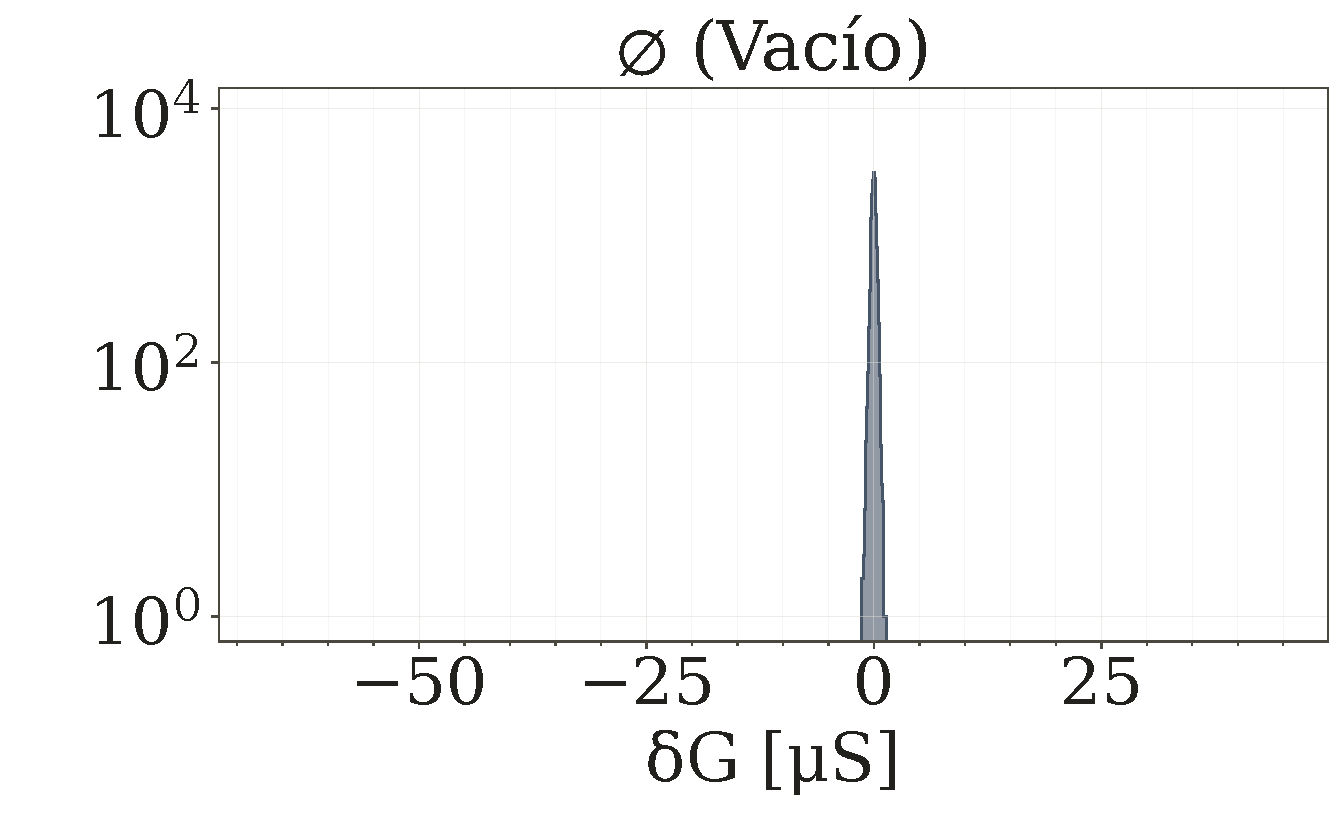
\includegraphics[width=0.48\textwidth]{Null_Histogram.pdf}\hfill
			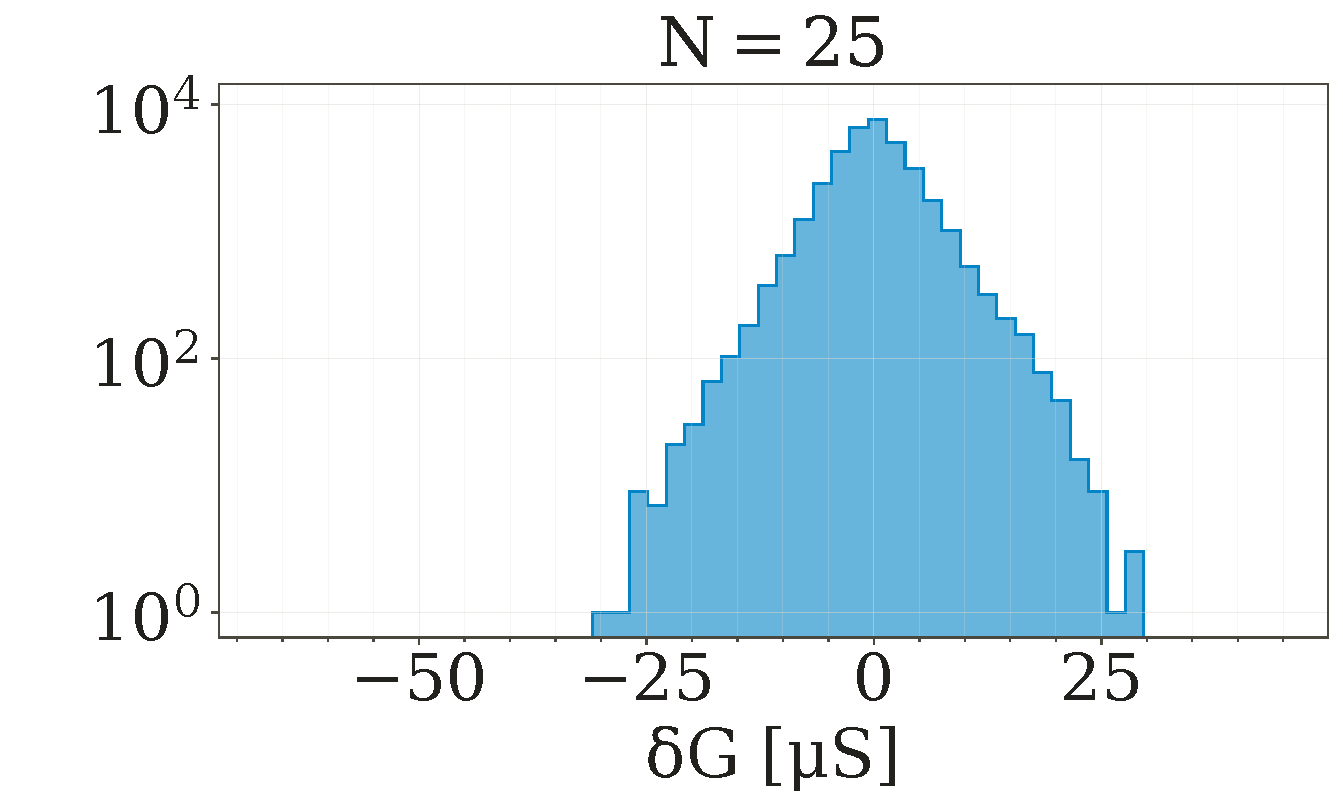
\includegraphics[width=0.48\textwidth]{Histogram_25.pdf}\\[0.5em]
			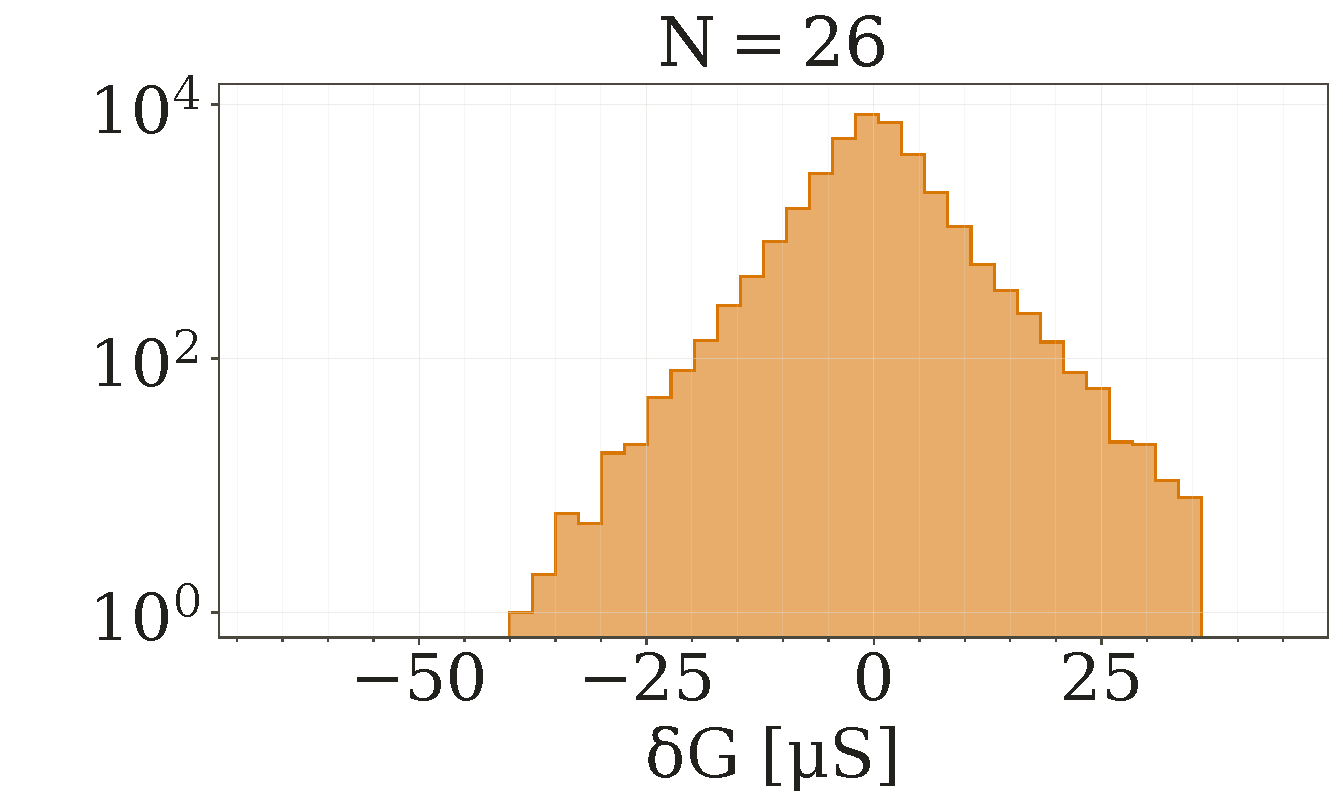
\includegraphics[width=0.48\textwidth]{Histogram_26.pdf}\hfill
			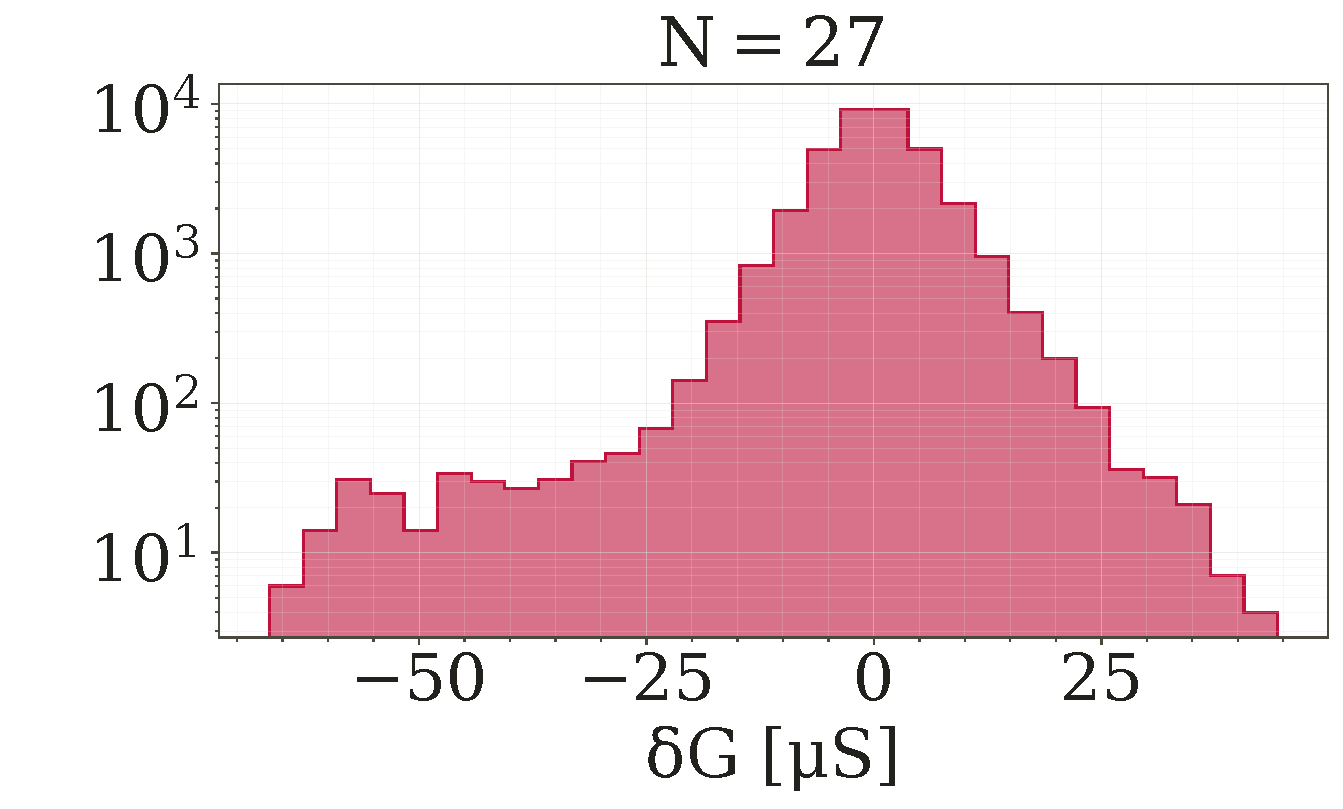
\includegraphics[width=0.48\textwidth]{Histogram_27.pdf}\\
			\vspace{0.4em}
			{\small \textit{Ventana temporal centrada exclusivamente en el máximo de asimetría direccional para la muestra más densa.}}
		\end{posterbox}
		
		\begin{posterbox}[name=asym_surv,column=2,span=4,below=hist]{B. Impactos Colectivos: Sincronización y Fuerzas Extremas}
			\begin{minipage}{0.48\textwidth}
				\centering
				\includegraphics[width=\textwidth]{"Skewness vs deltaT.pdf"}\\
				\vspace{0.2em}
				{\small \textit{Picos de asimetría evidencian empujones coordinados contra la pared.}}
			\end{minipage}
			\hfill
			\begin{minipage}{0.48\textwidth}
				\centering
				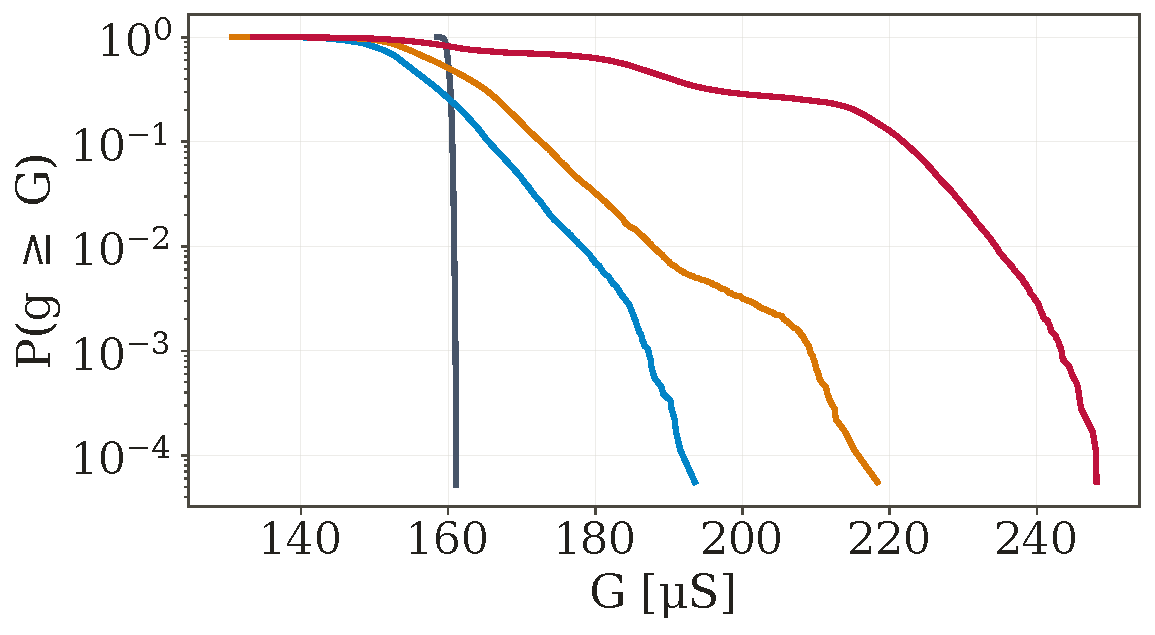
\includegraphics[width=\textwidth]{Supervivencia.pdf}\\
				\vspace{0.2em}
				{\small \textit{El decaimiento más lento de la cola revela impactos extremos frecuentes.}}
			\end{minipage}
		\end{posterbox}
		
		\begin{posterbox}[name=jamming,column=2,span=4,below=asym_surv]{C. Serie Temporal: El Ciclo de Jamming Activo}
			\centering
			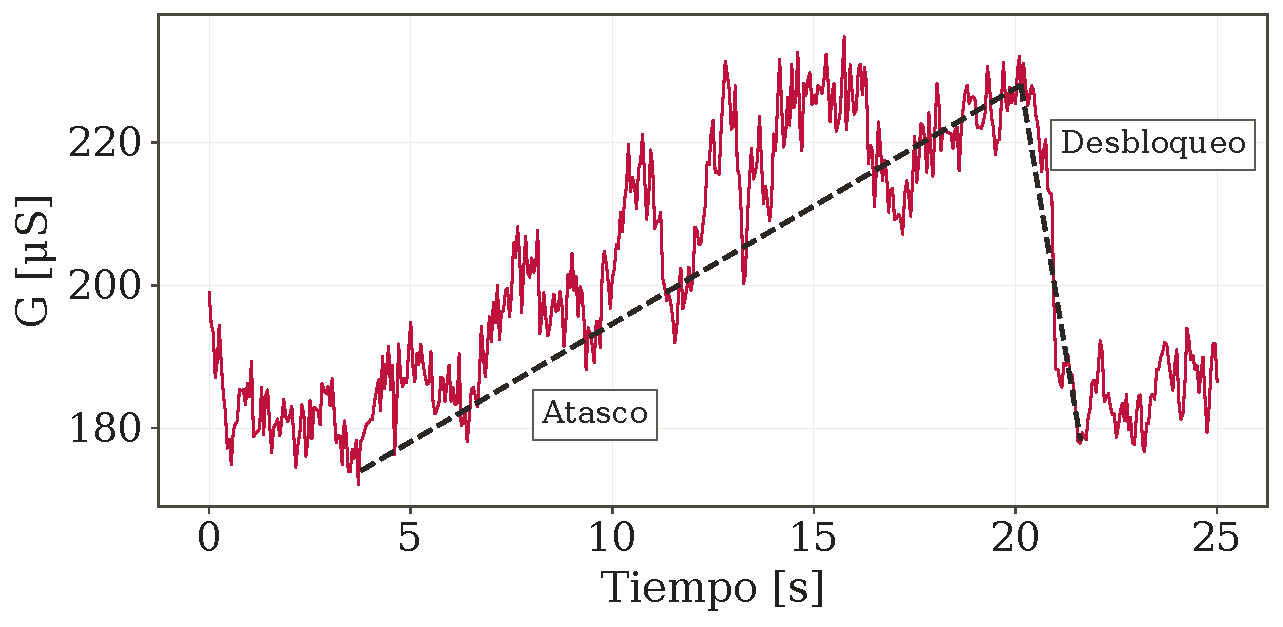
\includegraphics[width=0.75\textwidth]{Jamming.pdf}\\
			\vspace{0.2em}
			{\small \textit{Dinámica de atasco. La presión sube constantemente (arco bloqueado) y finaliza con una caída vertical abrupta (desatasco).}}
		\end{posterbox}
		
		\begin{posterbox}[name=concl,column=2,span=4,below=jamming,bottomaligned=refs]{4. CONCLUSIONES}
			\raggedright
			\large 
			\begin{itemize}[leftmargin=*, noitemsep]
				\item El sensor FSR permitió medir las fluctuaciones de fuerza con altísima resolución, validando una técnica de bajo costo para materia activa.
				\item A mayor densidad, la presión pierde homogeneidad: los impactos mecánicos colectivos se coordinan (picos de asimetría) y las fuerzas extremas aumentan drásticamente.
				\item Se logró capturar la firma mecánica del ciclo de \textit{jamming}: acumulación de presión por bloqueo estructural, seguida de un colapso abrupto.
			\end{itemize}
		\end{posterbox}
		
	\end{poster}
\end{document}